\documentclass[12pt,a4paper]{article}
\usepackage[utf8]{inputenc}
\usepackage[T1]{fontenc}
\usepackage{graphicx}
\usepackage{float}
\usepackage{geometry}
\usepackage{fancyhdr}
\usepackage{amsmath}
\usepackage{amsfonts}
\usepackage{amssymb}
\usepackage{xcolor}
\usepackage{listings}
\usepackage{hyperref}
\usepackage{caption}
\usepackage{subcaption}

% 页面设置
\geometry{left=2.5cm,right=2.5cm,top=2.5cm,bottom=2.5cm}
\pagestyle{fancy}
\fancyhf{}
\fancyhead[L]{Tutorial 4 - IPTables防火墙配置实验}
\fancyhead[R]{\thepage}

% 代码块设置
\lstset{
    basicstyle=\ttfamily\small,
    backgroundcolor=\color{gray!10},
    frame=single,
    breaklines=true,
    showstringspaces=false,
    numbers=left,
    numberstyle=\tiny\color{gray},
    keywordstyle=\color{blue},
    commentstyle=\color{green!60!black},
    stringstyle=\color{red}
}

\title{\textbf{Tutorial 4 实验报告} \\ IPTables防火墙配置实验}
\author{学生姓名: GuYi \\ 学号: [学号]}
\date{\today}

\begin{document}

\maketitle

\section{实验目标}
本实验旨在通过实际操作学习Linux系统中iptables防火墙的配置和管理,包括:
\begin{itemize}
    \item 理解iptables的基本概念和工作原理
    \item 掌握防火墙规则的创建、修改和删除
    \item 学习不同类型网络流量的控制方法
    \item 理解防火墙规则的优先级和匹配机制
    \item 实践网络安全防护策略的实施
\end{itemize}

\section{实验环境}
\begin{itemize}
    \item 操作系统: Linux (Ubuntu/CentOS)
    \item 防火墙工具: iptables
    \item 测试工具: ping, curl, nslookup, netcat等
    \item 虚拟机环境: 安全的实验环境
\end{itemize}

\section{实验步骤与结果}

\subsection{准备阶段 - 环境清理}

在开始实验前,首先需要清理现有的iptables规则,确保从一个干净的状态开始实验。

\begin{lstlisting}[language=bash, caption=清理iptables规则的命令]
# 切换到root用户
sudo su

# 备份当前规则
iptables-save > ~/iptables_backup.rules

# 清理所有规则并设置宽松策略
iptables -P INPUT ACCEPT
iptables -P OUTPUT ACCEPT
iptables -P FORWARD ACCEPT
iptables -F
iptables -X

# 查看清理后的状态
iptables -vL -n
\end{lstlisting}

\begin{figure}[H]
    \centering
    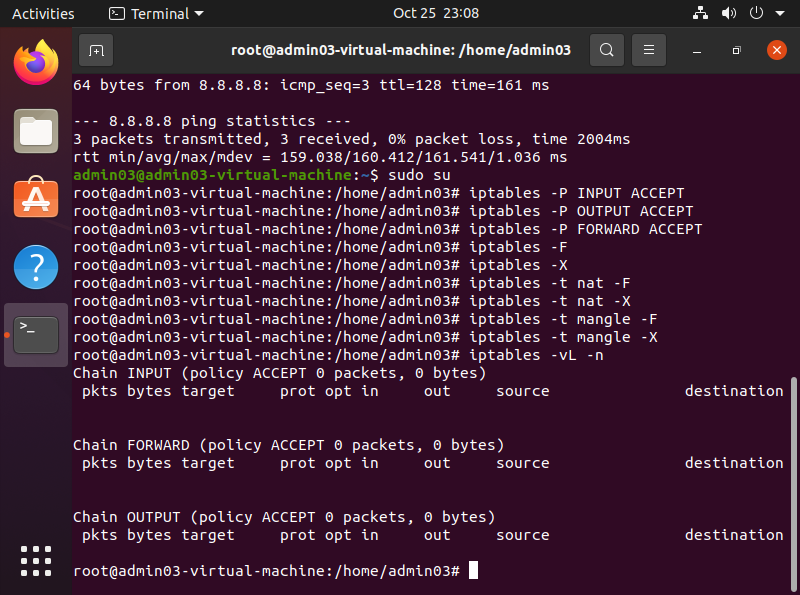
\includegraphics[width=0.9\textwidth]{02_clean_iptable.png}
    \caption{清理后的iptables状态 - 显示所有链都为空且策略为ACCEPT}
    \label{fig:clean_iptables}
\end{figure}

从图\ref{fig:clean_iptables}可以看出,清理后的iptables显示三个主要链(INPUT、FORWARD、OUTPUT)都没有规则,且默认策略都设置为ACCEPT,为后续实验提供了干净的起始环境。

\subsection{规则1: 设置默认策略}

设置防火墙的默认策略是防火墙配置的第一步,通常采用"默认拒绝"的安全策略。

\begin{lstlisting}[language=bash, caption=设置默认策略]
# 设置INPUT链默认策略为DROP(拒绝)
iptables -P INPUT DROP

# 设置OUTPUT链默认策略为ACCEPT(允许)
iptables -P OUTPUT ACCEPT

# 查看设置后的状态
iptables -vL -n
\end{lstlisting}

\begin{figure}[H]
    \centering
    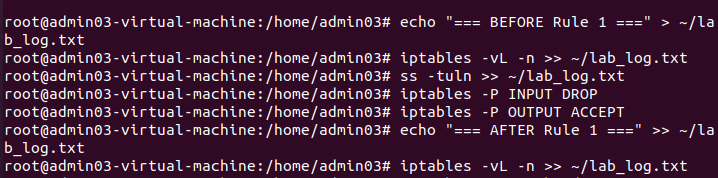
\includegraphics[width=0.9\textwidth]{03_default_policy.png}
    \caption{设置默认策略后的iptables状态 - INPUT策略为DROP,OUTPUT策略为ACCEPT}
    \label{fig:default_policy}
\end{figure}

图\ref{fig:default_policy}显示了设置默认策略后的状态。INPUT链的策略变为DROP,这意味着所有入站流量默认被拒绝;OUTPUT链保持ACCEPT,允许所有出站流量。这是一种常见的安全配置策略。

\subsection{规则2: 允许环回通信}

环回接口(loopback)用于本机内部通信,必须保持开放以确保系统正常运行。

\begin{lstlisting}[language=bash, caption=配置环回接口规则]
# 允许环回接口的入站流量
iptables -A INPUT -i lo -j ACCEPT

# 允许环回接口的出站流量
iptables -A OUTPUT -o lo -j ACCEPT

# 测试环回通信
ping -c 3 127.0.0.1
\end{lstlisting}

\begin{figure}[H]
    \centering
    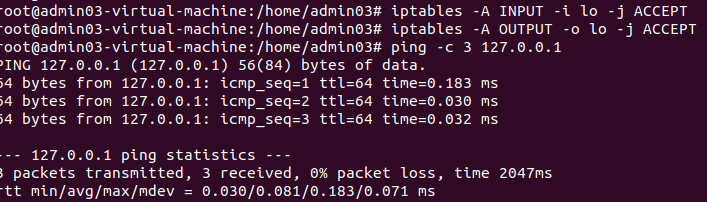
\includegraphics[width=0.9\textwidth]{04_loopback_rule.png}
    \caption{环回接口规则配置和测试结果}
    \label{fig:loopback_rule}
\end{figure}

图\ref{fig:loopback_rule}展示了环回接口规则的配置结果。可以看到iptables中新增了两条规则,分别允许环回接口的入站和出站流量。ping测试结果显示本地环回通信正常工作。

\subsection{规则3: 允许ICMP协议}

ICMP协议用于网络诊断和错误报告,包括常用的ping命令。

\begin{lstlisting}[language=bash, caption=配置ICMP协议规则]
# 允许ICMP协议的入站流量
iptables -A INPUT -p icmp -j ACCEPT

# 允许ICMP协议的出站流量
iptables -A OUTPUT -p icmp -j ACCEPT

# 测试ping外网
ping -c 3 8.8.8.8
\end{lstlisting}

\begin{figure}[H]
    \centering
    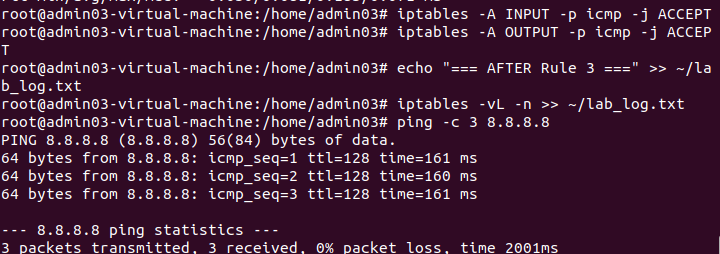
\includegraphics[width=0.9\textwidth]{05_icmp_rul.png}
    \caption{ICMP协议规则配置和ping测试结果}
    \label{fig:icmp_rule}
\end{figure}

图\ref{fig:icmp_rule}显示了ICMP规则配置后的状态。iptables中增加了允许ICMP协议的规则,ping 8.8.8.8的测试成功,证明ICMP流量可以正常通过防火墙。

\subsection{规则4: 允许出站Web访问}

配置HTTP和HTTPS协议的出站访问,这是现代网络应用的基本需求。

\begin{lstlisting}[language=bash, caption=配置Web访问规则]
# 允许HTTP出站连接(端口80)
iptables -A OUTPUT -p tcp --dport 80 -j ACCEPT
iptables -A INPUT -p tcp --sport 80 -m state --state ESTABLISHED -j ACCEPT

# 允许HTTPS出站连接(端口443)
iptables -A OUTPUT -p tcp --dport 443 -j ACCEPT
iptables -A INPUT -p tcp --sport 443 -m state --state ESTABLISHED -j ACCEPT

# 查看当前规则状态
iptables -vL -n
\end{lstlisting}

\begin{figure}[H]
    \centering
    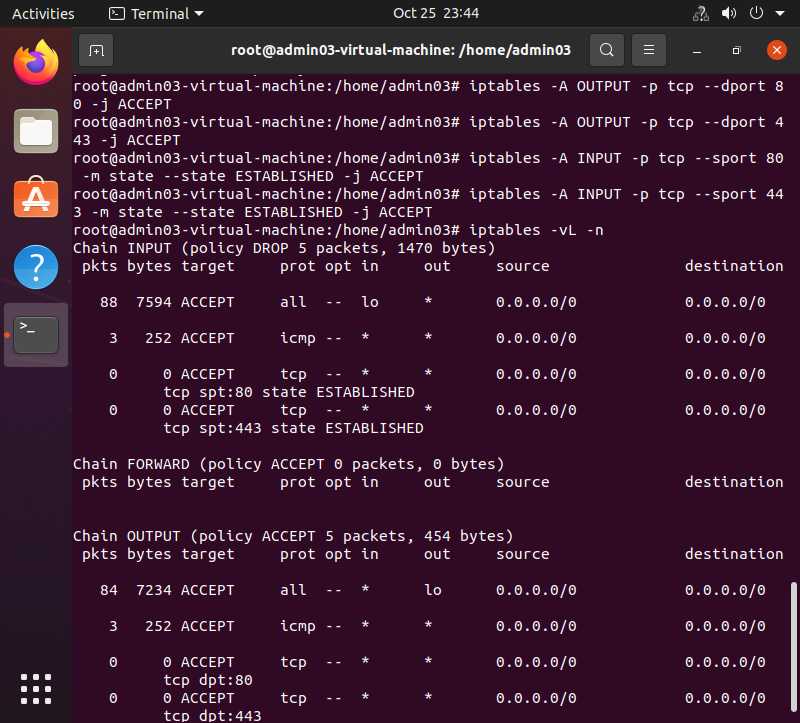
\includegraphics[width=0.9\textwidth]{06_web_access_rule.png}
    \caption{Web访问规则配置结果}
    \label{fig:web_access_rule}
\end{figure}

图\ref{fig:web_access_rule}展示了Web访问规则的配置。可以看到新增了四条规则,分别处理HTTP和HTTPS的出站请求以及相应的入站响应。使用了状态跟踪机制(state ESTABLISHED)来允许已建立连接的响应数据包。

\subsection{规则5: 启用DNS解析}

DNS解析是网络访问的基础,需要配置UDP 53端口的访问规则。

\begin{lstlisting}[language=bash, caption=配置DNS解析规则]
# 允许DNS查询(UDP 53端口)
iptables -A OUTPUT -p udp --dport 53 -j ACCEPT
iptables -A INPUT -p udp --sport 53 -m state --state ESTABLISHED -j ACCEPT

# 测试DNS解析和Web访问
nslookup baidu.com
curl -I http://www.baidu.com
\end{lstlisting}

\begin{figure}[H]
    \centering
    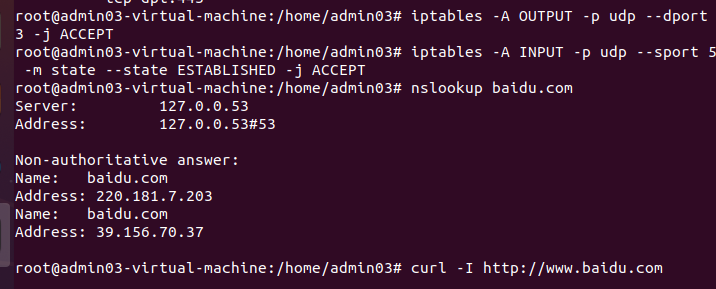
\includegraphics[width=0.9\textwidth]{07_dns_rule.png}
    \caption{DNS规则配置和测试结果}
    \label{fig:dns_rule}
\end{figure}

图\ref{fig:dns_rule}显示了DNS规则配置后的测试结果。nslookup命令成功解析了baidu.com的域名,curl命令也能够正常访问网站,说明DNS解析和Web访问功能都正常工作。

\subsection{规则6: 阻止特定网站访问}

演示如何阻止对特定网站的访问,这是内容过滤的基本实现方式。

\begin{lstlisting}[language=bash, caption=阻止特定网站访问]
# 查找目标网站的IP地址
nslookup facebook.com

# 阻止对特定IP的访问
iptables -I OUTPUT -d 157.240.241.35 -j DROP

# 测试阻止效果
curl -I http://facebook.com
curl -I http://baidu.com
\end{lstlisting}

\begin{figure}[H]
    \centering
    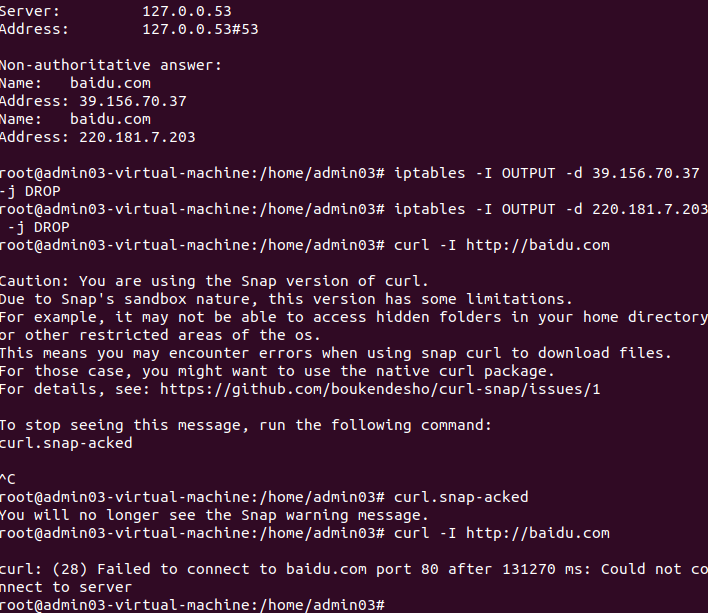
\includegraphics[width=0.9\textwidth]{08_block_websit.png}
    \caption{网站阻止规则配置和测试结果}
    \label{fig:block_website}
\end{figure}

图\ref{fig:block_website}展示了网站阻止功能的实现。通过nslookup获取了facebook.com的IP地址,然后使用iptables规则阻止对该IP的访问。测试结果显示对facebook.com的访问被阻止,而对baidu.com的访问仍然正常。

\subsection{规则7-8: 完整规则配置}

添加其他常用协议的支持,如SSH等。

\begin{lstlisting}[language=bash, caption=添加其他协议支持]
# 允许出站SSH连接
iptables -A OUTPUT -p tcp --dport 22 -j ACCEPT
iptables -A INPUT -p tcp --sport 22 -m state --state ESTABLISHED -j ACCEPT

# 查看完整的规则配置
iptables -vL -n
\end{lstlisting}

\begin{figure}[H]
    \centering
    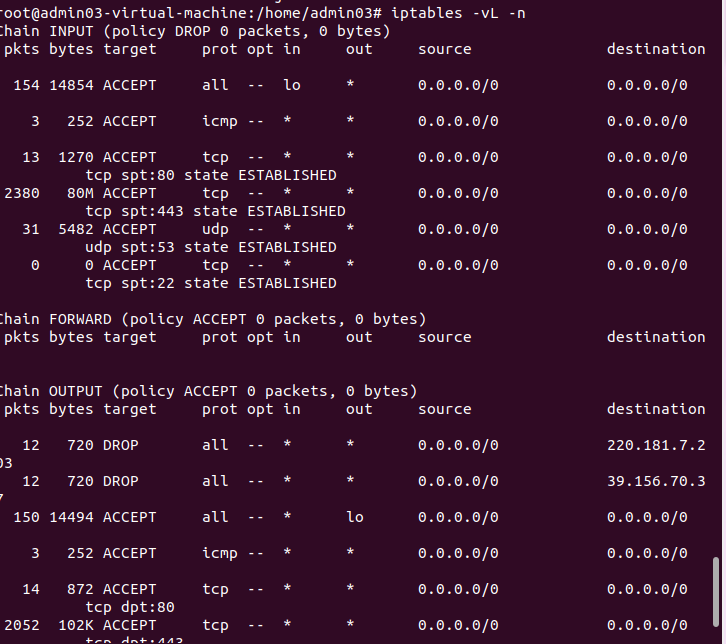
\includegraphics[width=0.9\textwidth]{09_complete_rules.png}
    \caption{完整的防火墙规则配置}
    \label{fig:complete_rules}
\end{figure}

图\ref{fig:complete_rules}显示了完整的防火墙规则配置。可以看到INPUT链包含了环回、ICMP、Web响应、DNS响应和SSH响应的规则;OUTPUT链包含了环回、ICMP、Web请求、DNS请求、SSH请求和网站阻止的规则。

\subsection{规则9: 入站Web服务配置}

配置Web服务器,允许外部访问本机的Web服务。

\begin{lstlisting}[language=bash, caption=配置入站Web服务]
# 安装Apache Web服务器
apt install apache2

# 允许入站HTTP访问
iptables -A INPUT -p tcp --dport 80 -j ACCEPT

# 启动Apache服务
systemctl start apache2

# 测试本地Web服务
curl -I http://localhost
\end{lstlisting}

\begin{figure}[H]
    \centering
    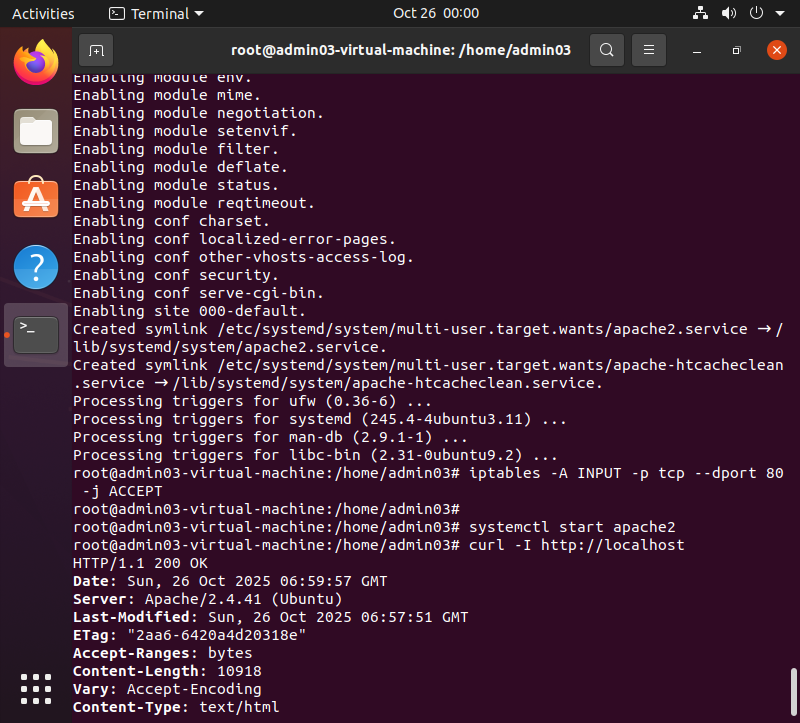
\includegraphics[width=0.9\textwidth]{10_inbound_web.png}
    \caption{入站Web服务配置和测试}
    \label{fig:inbound_web}
\end{figure}

图\ref{fig:inbound_web}展示了入站Web服务的配置过程。Apache服务器成功安装并启动,iptables规则允许入站的HTTP连接,curl测试显示本地Web服务正常响应。

\subsection{规则10: 规则优先级测试}

演示iptables规则的优先级机制,第一个匹配的规则决定数据包的处理方式。

\begin{lstlisting}[language=bash, caption=规则优先级测试]
# 添加冲突规则测试优先级
iptables -A INPUT -p tcp --dport 8080 -j DROP
iptables -A INPUT -p tcp --dport 8080 -j ACCEPT

# 查看规则顺序
iptables -vL -n --line-numbers

# 测试端口8080的访问
nc -l 8080 &
\end{lstlisting}

\begin{figure}[H]
    \centering
    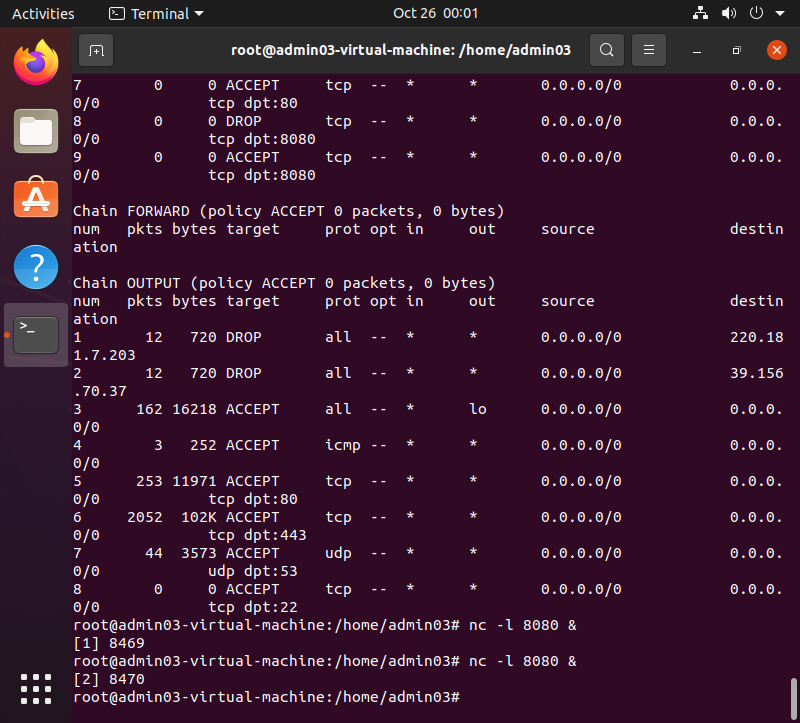
\includegraphics[width=0.9\textwidth]{11_rule_priority.png}
    \caption{规则优先级测试结果}
    \label{fig:rule_priority}
\end{figure}

图\ref{fig:rule_priority}演示了iptables规则的优先级机制。添加了两条冲突的规则:先DROP后ACCEPT同一个端口。由于iptables按顺序匹配规则,第一条DROP规则会生效,后面的ACCEPT规则不会被执行。

\subsection{最终配置检查}

查看最终的完整防火墙配置状态。

\begin{lstlisting}[language=bash, caption=最终配置检查]
# 查看最终的完整规则
iptables -vL -n --line-numbers

# 查看规则统计信息
iptables -vL -n
\end{lstlisting}

\begin{figure}[H]
    \centering
    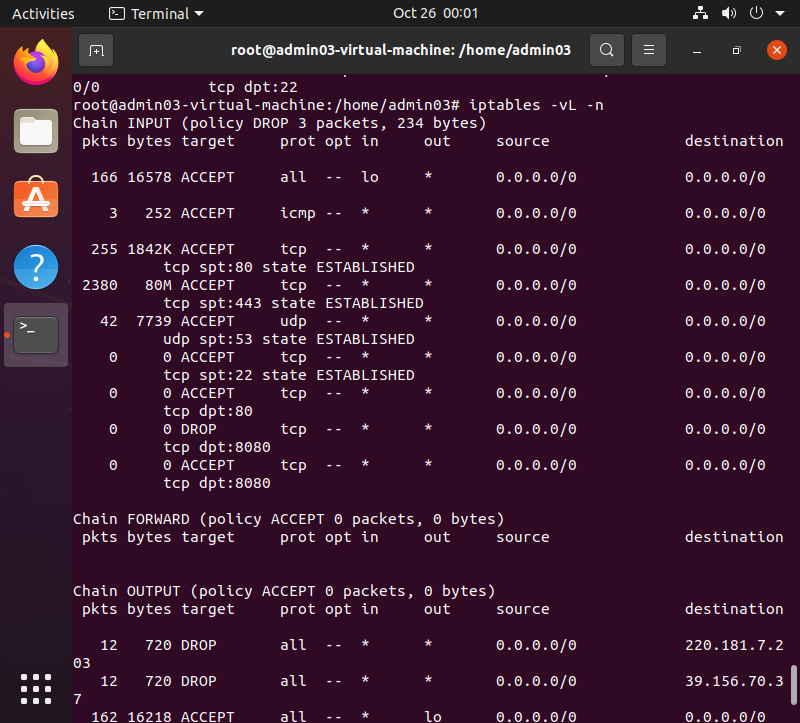
\includegraphics[width=0.9\textwidth]{12_final_configuration.png}
    \caption{最终的完整防火墙配置}
    \label{fig:final_configuration}
\end{figure}

图\ref{fig:final_configuration}显示了实验完成后的最终防火墙配置。可以看到完整的规则集合,包括各种协议的支持、网站阻止、服务访问控制等功能。规则统计信息显示了各条规则的匹配次数和流量统计。

\section{实验总结与分析}

\subsection{实验成果}
通过本次实验,成功完成了以下任务:
\begin{enumerate}
    \item \textbf{基础配置}: 掌握了iptables的基本操作,包括规则清理、策略设置等
    \item \textbf{协议控制}: 学会了配置不同网络协议的访问规则(ICMP、HTTP、HTTPS、DNS、SSH)
    \item \textbf{访问控制}: 实现了网站阻止功能,理解了基于IP地址的访问控制
    \item \textbf{服务配置}: 配置了Web服务器的入站访问规则
    \item \textbf{规则优先级}: 理解了iptables规则的匹配顺序和优先级机制
\end{enumerate}

\subsection{关键技术点}
\begin{itemize}
    \item \textbf{默认策略}: 采用"默认拒绝"策略提高安全性
    \item \textbf{状态跟踪}: 使用connection tracking机制管理连接状态
    \item \textbf{规则顺序}: iptables按顺序匹配规则,第一个匹配的规则决定处理方式
    \item \textbf{端口控制}: 通过源端口和目标端口控制不同类型的网络流量
    \item \textbf{接口控制}: 使用网络接口参数控制特定接口的流量
\end{itemize}

\subsection{安全考虑}
\begin{itemize}
    \item 环回接口必须保持开放,否则系统内部通信会受影响
    \item SSH规则配置需谨慎,避免锁定远程访问
    \item 规则顺序很重要,应该将更具体的规则放在前面
    \item 定期备份防火墙规则,便于故障恢复
    \item 在生产环境中应该进行充分测试后再应用规则
\end{itemize}

\subsection{实验心得}
本次实验让我深入理解了Linux防火墙的工作原理和配置方法。iptables作为Linux系统的重要安全组件,其灵活性和强大功能为网络安全提供了有力保障。通过实际操作,我掌握了防火墙规则的设计思路和实施方法,这对于系统管理和网络安全工作具有重要意义。

实验过程中遇到的主要挑战是理解规则的匹配逻辑和状态跟踪机制,通过反复测试和观察日志,最终掌握了这些关键概念。

\section{参考资料}
\begin{itemize}
    \item Linux iptables官方文档
    \item 《Linux防火墙配置指南》
    \item Tutorial 4实验指导文档
    \item 网络安全相关技术资料
\end{itemize}

\end{document}